%%%%%%%%%%%%%%%%%%%%%%%%%%%%%%%%%%%%%%%%%%%%%%%%%%%%%%%%%%%%%%%%%%%%%%%%%%%%%%%%
% \pi-Former: Succinct Proofs of Transformer Inference
% USENIX submission template (uses usenix-2020-09.sty).
%%%%%%%%%%%%%%%%%%%%%%%%%%%%%%%%%%%%%%%%%%%%%%%%%%%%%%%%%%%%%%%%%%%%%%%%%%%%%%%%

\documentclass[letterpaper,twocolumn,10pt]{article}
\usepackage{usenix-2020-09}

\usepackage{amsmath}
\usepackage{amssymb}
\usepackage{amsthm}
\usepackage{amsfonts}
\usepackage{bbm}
\usepackage{booktabs}
\usepackage{multirow}
\usepackage{algorithm}
\usepackage{algpseudocode}
\usepackage{tikz}
\usetikzlibrary{positioning,arrows.meta,calc,fit,backgrounds,shapes.geometric}
\usepackage{enumitem}
\setlist[itemize]{leftmargin=1.4em,topsep=2pt,itemsep=2pt}
\setlist[enumerate]{leftmargin=1.6em,topsep=2pt,itemsep=2pt}

\newtheorem{theorem}{Theorem}
\newtheorem{lemma}[theorem]{Lemma}
\newtheorem{proposition}[theorem]{Proposition}
\newtheorem{corollary}[theorem]{Corollary}
\theoremstyle{remark}
\newtheorem{remark}[theorem]{Remark}
\theoremstyle{definition}
\newtheorem{definition}[theorem]{Definition}

\algrenewcommand\algorithmicrequire{\textbf{Input:}}
\algrenewcommand\algorithmicensure{\textbf{Output:}}
\algnewcommand{\LineComment}[1]{\Statex \(\triangleright\) \emph{#1}}
\algnewcommand{\Phase}[1]{\Statex \textbf{Phase #1}}

\newcommand{\sys}{\ensuremath{\pi\text{-Former}}}
\newcommand{\FF}{\mathbb{F}}
\newcommand{\GG}{\mathbb{G}}
\newcommand{\RR}{\mathbb{R}}
\newcommand{\ZZ}{\mathbb{Z}}
\newcommand{\bphi}{\boldsymbol{\phi}}
\newcommand{\bq}{\mathbf{q}}
\newcommand{\bk}{\mathbf{k}}
\newcommand{\bv}{\mathbf{v}}
\newcommand{\bx}{\mathbf{x}}
\newcommand{\by}{\mathbf{y}}
\newcommand{\bo}{\mathbf{o}}
\newcommand{\bO}{\mathbf{O}}
\newcommand{\bA}{\mathbf{A}}
\newcommand{\bB}{\mathbf{B}}
\newcommand{\bb}{\mathbf{b}}
\newcommand{\bM}{\mathbf{M}}
\newcommand{\bN}{\mathbf{N}}
\newcommand{\bX}{\mathbf{X}}
\newcommand{\bY}{\mathbf{Y}}
\newcommand{\bW}{\mathbf{W}}
\newcommand{\bQ}{\mathbf{Q}}
\newcommand{\bK}{\mathbf{K}}
\newcommand{\bV}{\mathbf{V}}
\newcommand{\bbeta}{\boldsymbol{\beta}}
\newcommand{\bgamma}{\boldsymbol{\gamma}}
\newcommand{\calM}{\mathcal{M}}
\newcommand{\calT}{\mathcal{T}}
\newcommand{\calP}{\mathcal{P}}
\newcommand{\calV}{\mathcal{V}}
\newcommand{\calA}{\mathcal{A}}
\newcommand{\piproof}{\pi}
\newcommand{\bits}{B}
\newcommand{\chunks}{c}
\newcommand{\chunkbits}{m}
\newcommand{\polylog}{\mathrm{polylog}}
\newcommand{\poly}{\mathrm{poly}}
\newcommand{\softmax}{\mathrm{softmax}}
\newcommand{\eq}{\widetilde{\mathrm{eq}}}
\DeclareMathOperator{\LN}{LN}
\DeclareMathOperator{\GELU}{GELU}
\DeclareMathOperator{\Att}{Att}
\DeclareMathOperator{\Com}{\mathsf{Com}}
\DeclareMathOperator{\Open}{\mathsf{Open}}
\DeclareMathOperator{\Verify}{\mathsf{Verify}}
\DeclareMathOperator{\Prove}{\mathsf{Prove}}
\DeclareMathOperator{\Setup}{\mathsf{Setup}}
\DeclareMathOperator{\poppk}{\mathsf{pk}}
\DeclareMathOperator{\popvk}{\mathsf{vk}}

%don't want date printed
\date{}

\title{\Large \bf \sys{}: Succinct Proofs of Transformer Inference\\
       via a SNARK-Friendly Architecture}

\author{
{\rm Hideaki Takahashi}\\
Columbia University\\
\texttt{ht2673@columbia.edu}
}

\begin{document}

\maketitle

%-------------------------------------------------------------------------------
\begin{abstract}
%-------------------------------------------------------------------------------
Verifiable transformer inference lets an untrusted operator prove
that a posted output was produced by a committed model, without
revealing the weights. The obstacle is that a transformer block is
built from exactly the operations that finite-field SNARKs find
expensive: softmax, GeLU, LayerNorm, and dense projections. Prior
systems leave the model untouched and pay this cost on every block.

We present \sys{}, a succinct argument whose central design choice
is to co-design the \emph{model} so the proof system has nothing
expensive to absorb. Three architectural changes drive the design:
(i) softmax attention is replaced by a kernel attention whose feature
map is realised as an additively decomposed learnable lookup, so the
only non-arithmetic operation is a structured Lasso table look-up;
(ii) every projection is constrained to ternary entries scaled by a
per-layer scalar, eliminating all field multiplications from weight
contractions; and (iii) LayerNorm is reformulated as an integer
protocol provable through sumcheck and chunked range proofs. We build
a transparent BN254 SNARK on top with Hyrax commitments, batching
every per-block sub-protocol into a constant number of model-level
sumchecks, a globally shared range-multiplicity commitment, and a
zerocheck-folded inverse polynomial that removes $B\!\cdot\!C$ Hyrax
commitments per range bucket. Residual connections require no proof:
they are verified by linearity of the commitment scheme. We prove
end-to-end soundness under discrete log on BN254 G1 and implement a
complete prototype in $\sim$19k lines of Rust with a bit-identical
PyTorch training pipeline.
\end{abstract}

%-------------------------------------------------------------------------------
\section{Introduction}
\label{sec:intro}
%-------------------------------------------------------------------------------

Large language models are increasingly deployed as black-box
services. The user submits a prompt, an opaque operator runs a
proprietary model, and the user has no cryptographic guarantee that
the returned output came from the advertised model. Verifiable
inference~\cite{liu2021zkcnn,sun2024zkllm,qu2025zkgpt,abbaszadeh2024zero}
closes this gap with a succinct non-interactive argument: the
operator commits to the weights once, and for every input produces a
small proof that the verifier checks without re-executing the model
and without learning the weights.

The core difficulty is that a transformer block is built from
operations that finite-field SNARKs find expensive. Softmax requires
exponentials and a row-wise division; GeLU is transcendental;
LayerNorm contains a square root and a division by a running
variance; a dense projection costs one field multiplication per
weight entry. Prior work attacks this on the proof-system side:
zkLLM~\cite{sun2024zkllm} introduces \texttt{tlookup}, a parallelised
lookup argument tailored to softmax and SwiGLU; zkGPT~\cite{qu2025zkgpt}
pairs Plonky2 with constraint fusion to drive down the cost of
approximating softmax. Both keep the model fixed and pay an
``unfriendly-operation tax'' on every block.

\paragraph{Our approach.}
\sys{} starts from a different premise: change the \emph{model} so
that the proof system has nothing expensive to absorb. Three
architectural principles drive the design:
\begin{itemize}
  \item \textbf{SNARK-friendly operators.} Replace every operation
        without a compact arithmetic representation. Softmax becomes
        a kernel attention whose only non-arithmetic component is a
        structured table lookup; LayerNorm becomes an integer
        protocol provable by sumcheck plus chunked range proofs.
  \item \textbf{Ternary projections for free contractions.}
        Constrain every projection matrix to entries
        $\{-1,0,+1\}$ scaled by a per-layer scalar
        $\alpha$~\cite{ma2025bitnet}. A degree-$2$ sumcheck against
        a ternary weight folds the equality polynomial against
        ternary entries with $+\!=$/$-\!=$/skip; no field
        multiplications appear in the contraction.
  \item \textbf{Learnable lookup tables.} The element-wise
        non-linearity $\bphi$ is itself learnable: it is parametrised
        as a sum of small sub-tables and trained end-to-end. Under
        Lasso~\cite{setty2024unlocking}, prover cost depends only on
        table size and query count, not on table contents, so
        training adapts table values at zero proving cost.
\end{itemize}
Together these reduce a transformer block to operations that map
directly to a low-degree sumcheck or to a Lasso lookup over a small
structured table.

\paragraph{Model-level batching.}
On top of this architecture we build a proof system around a single
observation: the same protocol runs once per block with independent
inputs but identical structure. \sys{} runs six model-level
sumchecks (one per protocol type) that fold all $L$ per-block claims
via a Fiat--Shamir random linear combination; the inner sumcheck
transcript is shared across blocks. The same idea applies to Lasso
(one global multi-instance proof per lookup family), to range checks
(one shared multiplicity commitment per width bucket spanning the
entire model), to residuals (homomorphic Hyrax addition; no proof at
all), and to the final opening stage (deferred batch accumulators
finalised in one MSM pair per parameter group). For the range proof
specifically, we replace the explicit Hyrax commitment to each LogUp
inverse polynomial by a zerocheck folded into the bucket sumcheck;
this removes $B\cdot C$ commitments per bucket without changing the
per-round prover cost.

\paragraph{Contributions.}
\begin{enumerate}
  \item A SNARK-friendly transformer block
        (\S\ref{sec:arch}) in which attention, normalisation, and
        projection each map to a sumcheck or a Lasso lookup, combining
        learnable lookup attention, ternary projections, and a
        constraint-fused integer LayerNorm.
  \item A complete protocol (\S\ref{sec:protocol}) batching all
        $L$ per-block sub-proofs into six model-level cross-block
        sumchecks, one global Lasso for the $\bphi$ family, and a
        bucket-batched range proof shared across the whole model.
  \item A zerocheck-folded LogUp range proof (\S\ref{ssec:range},
        Theorem~\ref{thm:range}) that eliminates $B\cdot C$
        Hyrax commitments per width bucket while keeping the
        bucket sumcheck cubic and soundness within $O(n/|\FF|)$.
  \item End-to-end soundness (\S\ref{sec:soundness},
        Theorem~\ref{thm:end-to-end}) reducing to discrete log on
        BN254 G1, and a working prototype in $\sim$19k Rust LoC with
        a bit-identical PyTorch training pipeline
        (\S\ref{sec:impl}).
\end{enumerate}

\paragraph{Threat model.}
We target the standard non-interactive argument-of-knowledge setting
in the random-oracle model. The verifier holds a verifying key
$\popvk$ binding the weights and lookup tables, a public input
$\bx_{\mathrm{in}}$, and a claimed output $\by$, and accepts iff
$\calM_\theta(\bx_{\mathrm{in}})\!=\!\by$ for the committed model.
Soundness is computational under discrete log on BN254 G1, the
standard assumption for the Hyrax PCS~\cite{wahby2018doubly}. The
current implementation is not zero-knowledge: weight commitments are
public and intermediate sumcheck evaluations are revealed. The
standard masking extension is discussed in \S\ref{sec:disc}.

%-------------------------------------------------------------------------------
\section{Preliminaries}
\label{sec:bg}
%-------------------------------------------------------------------------------

\paragraph{Notation.}
We work over the BN254 scalar field $\FF$ ($r\!\approx\!2^{254}$) and
the BN254 G1 group $\GG$. We use $L$ for the number of blocks, $T$
for the sequence length, $d$ for the embedding dimension, and $d_{ff}$
for the FFN width; the prototype is single-head ($d_h\!=\!d$). A
multilinear polynomial $\widetilde f$ on $n$ variables is identified
with its $2^n$ evaluations on $\{0,1\}^n$, and the equality polynomial
$\eq(r,x)\!=\!\prod_i(r_i x_i+(1\!-\!r_i)(1\!-\!x_i))$ satisfies
$\sum_x\eq(r,x)\widetilde f(x)=\widetilde f(r)$. Real-valued tensors are
quantised to integers and embedded in $\FF$ before commitment; our
training pipeline runs the same integer arithmetic, so the exported
witness matches the field circuit bit-for-bit.

\paragraph{Transformer block.}
A pre-norm block~\cite{vaswani2017attention} computes
$\bX_{\mathrm{mid}}\!=\!\bX_{\mathrm{in}}+\Att(\LN(\bX_{\mathrm{in}}))$ and
$\bX_{\mathrm{out}}\!=\!\bX_{\mathrm{mid}}+\mathrm{FFN}(\LN(\bX_{\mathrm{mid}}))$,
with softmax attention $\softmax(\bQ\bK^\top\!/\sqrt d)\bV$ and
LayerNorm~\cite{ba2016layer}
$\bgamma\!\odot\!(\bx-\mu)/\sqrt{\sigma^2+\epsilon}+\bbeta$. The
non-arithmetic primitives (exp, division, square root) dominate SNARK
complexity in prior work.

\paragraph{Sumcheck.}
The sumcheck protocol~\cite{setty2020spartan,thaler2022proofs} reduces a
claim $H\!=\!\sum_{x\in\{0,1\}^n}\!f(x)$ for an MLE $f$ of individual
degree $\delta$ to a single evaluation $f(r)$ at random $r$, with
soundness error $\le n\delta/|\FF|$ and verifier cost $O(n\delta)$.
\sys{} uses the degree-2 variant for products of two MLEs, the cubic
variant for LayerNorm variance and our zerocheck-folded range proof,
and a multi-batched variant $\sum_k\lambda_k\sum_x f_k(x)g_k(x)$ for
cross-block batching.

\paragraph{Hyrax PCS.}
Hyrax~\cite{wahby2018doubly} arranges $2^n\!=\!2^{\nu+\sigma}$ MLE
evaluations as a $2^\nu\!\times\!2^\sigma$ matrix and commits to each
row via a vector Pedersen commitment over transparent generators. The
scheme is computationally binding under DL on $\GG$, requires no trusted
setup, and gives $O(\sqrt N)$ commitments, openings, and proof size.
Crucially, the row-Pedersen structure is linear:
$\Com(\bA)\!+\!\Com(\bB)\!=\!\Com(\bA\!+\!\bB)$, which \sys{} exploits to
verify residual connections without any proof.

\paragraph{Lasso.}
\label{ssec:lasso}
Lasso~\cite{setty2024unlocking,arun2024jolt,fomenko2025understanding}
proves that $N$ queries are consistent with a public sub-table
$T\!\in\!\FF^{2^m}$ via one batched sumcheck. A composite table that
decomposes \emph{additively} into $c$ sub-tables (Lasso's structured
condition) is committed as $c$ small tables of size $2^{B/c}$. Lasso's
defining property for our design is that prover and verifier cost
depend on table size and query count, but are independent of table
\emph{contents}: training the entries of $T$ has zero proving-cost
impact.

%-------------------------------------------------------------------------------
\section{The \sys{} Architecture}
\label{sec:arch}
%-------------------------------------------------------------------------------

\begin{figure*}[t]
\centering
\resizebox{\textwidth}{!}{%
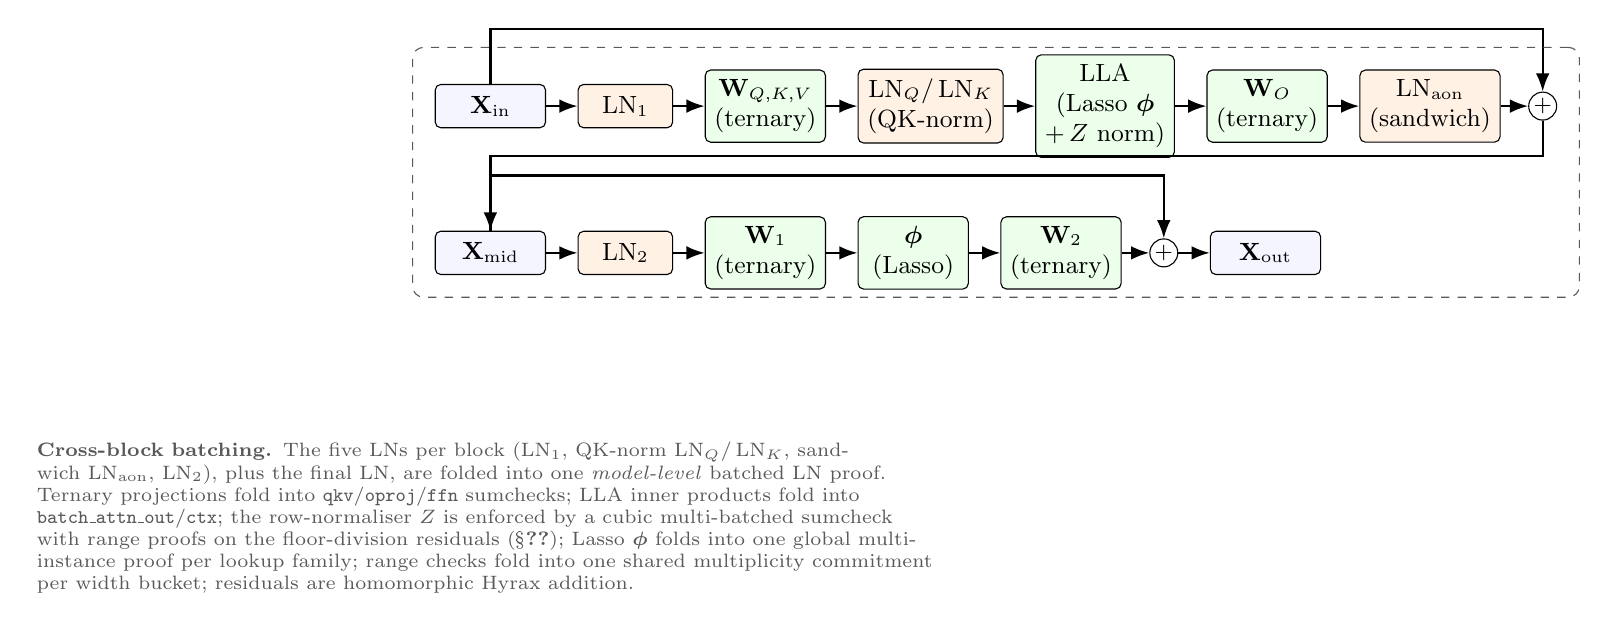
\begin{tikzpicture}[
    font=\small,
    box/.style={rectangle, draw, rounded corners=2pt, minimum width=1.4cm,
                minimum height=0.55cm, align=center, fill=blue!4},
    op/.style={rectangle, draw, rounded corners=2pt, minimum width=1.4cm,
               minimum height=0.55cm, align=center, fill=green!8},
    ln/.style={rectangle, draw, rounded corners=2pt, minimum width=1.2cm,
               minimum height=0.55cm, align=center, fill=orange!10},
    add/.style={circle, draw, inner sep=0.5pt, font=\footnotesize, fill=white},
    arrow/.style={-Latex, thick},
    label/.style={font=\scriptsize, color=gray!70!black}
  ]
  % ----- Top row: attention sub-block -----
  \node[box] (xin) at (0,0) {$\bX_{\mathrm{in}}$};
  \node[ln,  right=0.4cm of xin]   (ln1)  {$\LN_1$};
  \node[op,  right=0.4cm of ln1]   (qkv)  {$\bW_{Q,K,V}$\\(ternary)};
  \node[ln,  right=0.4cm of qkv]   (qkn)  {$\LN_{Q}\!/\LN_{K}$\\(QK-norm)};
  \node[op,  right=0.4cm of qkn]   (lla)  {LLA\\(Lasso $\bphi$\\$+\,Z$ norm)};
  \node[op,  right=0.4cm of lla]   (woo)  {$\bW_O$\\(ternary)};
  \node[ln,  right=0.4cm of woo]   (aon)  {$\LN_{\mathrm{aon}}$\\(sandwich)};
  \node[add, right=0.35cm of aon]  (res1) {$+$};
  \draw[arrow] (xin.east) -- (ln1.west);
  \draw[arrow] (ln1.east) -- (qkv.west);
  \draw[arrow] (qkv.east) -- (qkn.west);
  \draw[arrow] (qkn.east) -- (lla.west);
  \draw[arrow] (lla.east) -- (woo.west);
  \draw[arrow] (woo.east) -- (aon.west);
  \draw[arrow] (aon.east) -- (res1.west);
  \draw[arrow] (xin.north) |- ($(xin.north)+(0,0.7)$) -| (res1.north);

  % ----- Bottom row: FFN sub-block -----
  \node[box,  below=1.3cm of xin]    (xmid) {$\bX_{\mathrm{mid}}$};
  \node[ln,   right=0.4cm of xmid]   (ln2)  {$\LN_2$};
  \node[op,   right=0.4cm of ln2]    (w1)   {$\bW_1$\\(ternary)};
  \node[op,   right=0.4cm of w1]     (phi)  {$\bphi$\\(Lasso)};
  \node[op,   right=0.4cm of phi]    (w2)   {$\bW_2$\\(ternary)};
  \node[add,  right=0.35cm of w2]    (res2) {$+$};
  \node[box,  right=0.4cm of res2]   (xout) {$\bX_{\mathrm{out}}$};
  \draw[arrow] (xmid.east) -- (ln2.west);
  \draw[arrow] (ln2.east)  -- (w1.west);
  \draw[arrow] (w1.east)   -- (phi.west);
  \draw[arrow] (phi.east)  -- (w2.west);
  \draw[arrow] (w2.east)   -- (res2.west);
  \draw[arrow] (res2.east) -- (xout.west);
  \draw[arrow] (xmid.north) |- ($(xmid.north)+(0,0.7)$) -| (res2.north);
  \draw[arrow] (res1.south) |- ($(res1.south)+(0,-0.45)$) -| (xmid.north);

  \node[draw, dashed, rounded corners,
        fit=(ln1)(aon)(res1)(xmid)(xout)(res2),
        inner sep=8pt, label={[label]above:Single \sys{} block (one of $L$);\;5 LayerNorms (orange)}] {};
  \node[font=\scriptsize, color=gray!70!black, below=2.0cm of xmid,
        align=left, text width=0.95\textwidth] (note) {%
    \textbf{Cross-block batching.} The five LNs per block (LN$_1$,
    QK-norm $\LN_Q\!/\LN_K$, sandwich $\LN_{\mathrm{aon}}$, LN$_2$),
    plus the final LN, are folded into one
    \emph{model-level} batched LN proof. Ternary projections fold into
    \texttt{qkv}/\texttt{oproj}/\texttt{ffn} sumchecks; LLA inner products
    fold into \texttt{batch\_attn\_out}/\texttt{ctx}; the row-normaliser $Z$
    is enforced by a cubic multi-batched sumcheck with range proofs on the
    floor-division residuals (\S\ref{ssec:LLA}); Lasso $\bphi$ folds into
    one global multi-instance proof per lookup family; range checks fold
    into one shared multiplicity commitment per width bucket;
    residuals are homomorphic Hyrax addition.
  };
\end{tikzpicture}}
\caption{A single \sys{} block. Boxes are matrices; rounded green nodes are
operations the SNARK proves; orange nodes are LayerNorms. \emph{Sandwich
norm} ($\LN_{\mathrm{aon}}$) is applied to the attention output before the
residual; \emph{QK-norm} ($\LN_Q$, $\LN_K$) is applied to $\bQ,\bK$ after the
ternary projection and before $\bphi$. Ternary projections contain no field
multiplications in the contraction; Lasso lookup cost is independent of
table contents; residual $+$ is checked by homomorphic addition of Hyrax
commitments and requires no proof.}
\label{fig:block}
\end{figure*}

A \sys{} block (Figure~\ref{fig:block}) is a sandwich-normalised
linear-attention block. With $\bX_{\mathrm{in}}\!\in\!\FF^{T\times d}$,
the block computes
\begin{align*}
  \bX_{\mathrm{n1}}      &= \LN_1(\bX_{\mathrm{in}}),\\
  \bQ,\bK,\bV           &= \bX_{\mathrm{n1}}\bW_{Q,K,V} \;\;\text{(ternary)},\\
  \bQ^{\mathrm{n}},\bK^{\mathrm{n}} &= \LN_Q(\bQ),\;\LN_K(\bK),\\
  \bN                   &= \bphi(\bQ^{\mathrm{n}})\bigl(\bphi(\bK^{\mathrm{n}})^\top\bV\bigr),\\
  Z_t                   &= \bphi(\bq_t^{\mathrm{n}})^{\!\top}\!{\textstyle\sum_s}\bphi(\bk_s^{\mathrm{n}}),\\
  \bY^{\mathrm{att}}_{tj}&= \lfloor S\!\cdot\!\bN_{tj}/Z_t\rfloor,\\
  \bX_{\mathrm{mid}}    &= \bX_{\mathrm{in}} + \LN_{\mathrm{aon}}(\bY^{\mathrm{att}}\bW_O+\bb_O),\\
  \bX_{\mathrm{out}}    &= \bX_{\mathrm{mid}} + \bphi(\LN_2(\bX_{\mathrm{mid}})\bW_1)\bW_2.
\end{align*}
After $L$ such blocks the model applies a final LayerNorm and a
ternary LM head; the model contains $5L\!+\!1$ LayerNorms in total.
The scale $S$ re-introduces fractional precision before the integer
floor division.

Two of the five LayerNorms per block are not in a textbook
transformer but are essential for our integer pipeline.
\emph{QK-norm} ($\LN_Q,\LN_K$) pins the range of $\bQ,\bK$ so that
$\bphi(\bQ^{\mathrm n}),\bphi(\bK^{\mathrm n})$ and $Z$ stay in the
lookup-table range under any per-layer ternary scale.
\emph{Sandwich norm} ($\LN_{\mathrm{aon}}$) absorbs the unbounded
magnitude of linear attention before the residual: softmax is
row-stochastic and naturally bounded, but
$\bphi(\bQ)(\bphi(\bK)^\top\bV)$ is not, and an unnormalised residual
destabilises downstream LayerNorms. Both share one LN sub-protocol
(\S\ref{ssec:ln}); their only cost is extra LN witnesses, folded into
the model-level batched LN proof and the bucketed range batch.

\subsection{Learnable Lookup Attention}
\label{ssec:LLA}

Softmax attention requires $T^2$ exponentials and $T$ row-wise
divisions. We replace the kernel with a positive-definite inner
product $\kappa(\bq,\bk)\!=\!\langle\bphi(\bq),\bphi(\bk)\rangle$ on
the post-QK-norm tensors, where $\bphi\!:\!\RR^{d_h}\!\to\!\RR^{d_h}$
is an element-wise structured lookup (\S\ref{ssec:phi}). The block
computes the numerator
$\bN_{tj}\!=\!\bphi(\bq_t^{\mathrm{n}})^\top\!(\sum_s\bphi(\bk_s^{\mathrm{n}})\bv_s^\top)_j$
and the per-row denominator
$Z_t\!=\!\bphi(\bq_t^{\mathrm{n}})^\top\!\sum_s\bphi(\bk_s^{\mathrm{n}})$.
The context matrix
$\bM\!=\!\sum_s\bphi(\bk_s^{\mathrm{n}})\bv_s^\top\!\in\!\FF^{d_h\times d_h}$
is computed once per block, giving $O(T d_h^2)$ prover cost instead of
$O(T^2 d_h)$~\cite{katharopoulos2020transformers}.

\paragraph{Floor-division proof for row normalisation.}
\sys{} proves $\bY^{\mathrm{att}}_{tj}\!=\!\lfloor S\bN_{tj}/Z_t\rfloor$
in-circuit. The witness includes auxiliary tensors $\mathrm{rem}$ and
$\mathrm{diff}$ with $\mathrm{rem}_{tj}\!=\!S\bN_{tj}\!-\!Z_t\bY^{\mathrm{att}}_{tj}$
and $\mathrm{diff}_{tj}\!=\!Z_t\!-\!1\!-\!\mathrm{rem}_{tj}$, all
committed via Hyrax. At a random
$r_{\mathrm{norm}}\!\in\!\FF^{t_{\mathrm{bits}}+d_{\mathrm{bits}}}$ one
cubic multi-batched sumcheck merges
$S\bN-\mathrm{rem}-Z\bY^{\mathrm{att}}=0$ and
$\lambda(Z-1-\mathrm{rem}-\mathrm{diff})=0$ under a Fiat--Shamir
scalar $\lambda$. Range proofs on $\mathrm{rem},\mathrm{diff}$ (in the
64-bit bucket of \S\ref{ssec:range}) enforce both to be non-negative,
which combined with the second identity gives
$0\!\le\!\mathrm{rem}\!<\!Z$~--- the unique floor-division witness. A
second sumcheck binds $Z_t$ to the committed
$\bphi(\bQ^{\mathrm n}),\bphi(\bK^{\mathrm n})$; a causal variant
binds $Z$ to a prefix sum.

\paragraph{Binding lookups to post-norm tensors.}
The Lasso queries for $\bphi$ are evaluated on $\bQ^{\mathrm n},\bK^{\mathrm n}$,
not the pre-norm $\bQ,\bK$. The prover commits both
$C_{\bQ},C_{\bK}$ (used by the QKV sumcheck) and
$C_{\bQ^{\mathrm n}},C_{\bK^{\mathrm n}}$ (used as $\bphi$ inputs); the
global $\bphi$ Lasso binds its query indices to the post-norm commitments
via one shared Hyrax batch open, and the LN sub-proof for $\LN_Q,\LN_K$
ties pre- and post-norm together.

\subsection{Additive sub-table feature map}
\label{ssec:phi}

Rather than fix a kernel, \sys{} parametrises $\bphi$ as a sum of
learnable sub-table lookups. With input bit-width $\bits$, decomposition
depth $\chunks\!\mid\!\bits$, and chunk width
$\chunkbits\!=\!\bits/\chunks$, define the integer index
$x_{\mathrm{int}}\!=\!\mathrm{clamp}(\lfloor x/s\rfloor,0,2^{\bits}\!-\!1)$
and chunk extractor
$\chi_i(x_{\mathrm{int}})\!=\!(x_{\mathrm{int}}\!\gg\!i\chunkbits)\,\&\,(2^{\chunkbits}\!-\!1)$.
Then
\begin{equation}
  \bphi(x) \;=\; \sum_{i=0}^{\chunks-1} T_i\bigl[\chi_i(x_{\mathrm{int}})\bigr],
  \label{eq:phi}
\end{equation}
where $T_0,\dots,T_{\chunks-1}\!\in\!\RR^{2^{\chunkbits}}$ are
learnable sub-tables. They are initialised so $\sum_i T_i\!\approx\!\GELU$
and trained end-to-end via the straight-through
estimator~\cite{bengio2013estimating}. For $\bits\!=\!16,\chunks\!=\!2$
this replaces a $65{,}536$-entry monolithic table with two $256$-entry
sub-tables, matching Lasso's structured-decomposability condition
(\S\ref{ssec:lasso}). Because Lasso prover cost is independent of table
values, training the entries of every $T_i$ end-to-end imposes zero
proving-cost penalty.

\subsection{Ternary projections}
\label{ssec:ternary}
Following BitNet b1.58~\cite{ma2025bitnet}, every projection matrix
($\bW_Q,\bW_K,\bW_V,\bW_O,\bW_1,\bW_2$, and the LM head) is constrained
to entries in $\calT=\{-1,0,+1\}$ scaled by a learnable per-layer
scalar $\alpha\!\in\!\FF$, so the forward pass is
$\by\!=\!\alpha(\bx\bW)+\bb$ with $\bW\!\in\!\calT^{m\times n}$.
Training uses the magnitude-thresholded
$w\!\mapsto\!\mathrm{sign}(w)\!\cdot\![|w|\!>\!0.7\overline{|w|}]$ map
with the straight-through estimator; $\alpha$ is multiplied in after
the matrix product so the in-circuit weight stays ternary.

In the SNARK, the contraction $\bY(r_t,r_d)\!-\!\bb(r_d)\!=\!\alpha\sum_k\bX(r_t,k)\bW(k,r_d)$
is a degree-2 sumcheck that materialises only the cheap vector
$\alpha\!\cdot\!\bW(\cdot,r_d)$. The prover folds the equality polynomial
against ternary entries with $+\!=$/$-\!=$/skip; no field multiplication
appears in the contraction.

\subsection{Constraint-fused LayerNorm}
\label{ssec:ln}
Let $\bx\!\in\!\ZZ^d$ be a row,
$\mathrm{sum\_x}\!=\!\sum_j x_j$,
$\mathrm{sq\_sum\_x}\!=\!\sum_j x_j^2$, and
$\sigma\!=\!\lfloor\sqrt{\mathrm{var\_x}}/d\rfloor$. The integer variance
is $\mathrm{var\_x}\!=\!d(d\,\mathrm{sq\_sum\_x}-\mathrm{sum\_x}^2)$,
which expands $\sum_j(d x_j-\mathrm{sum\_x})^2$ without taking
$\mathrm{sum\_x}^2$ outside the sumcheck. \sys{} proves a LayerNorm
without divisions or square roots in five sub-protocols:
\begin{enumerate}
  \item \textbf{Mean} (degree-2 sumcheck for $\widetilde{\mathrm{sum\_x}}$).
  \item \textbf{Square-sum} (cubic sumcheck for
        $\widetilde{\mathrm{sq\_sum\_x}}(r_t)\!=\!\sum_j x_{\mathrm{col}}(j)^3$
        with three copies of $x_{\mathrm{col}}$, keeping the round
        polynomial cubic).
  \item \textbf{Sigma residual} (cubic multi-batched sumcheck combining
        $\sum_i\eq\widetilde{\mathrm{sum\_x}}(i)^2$ and
        $\sum_i\eq(d\widetilde\sigma(i))^2$ under a Fiat--Shamir scalar
        $\lambda_{\mathrm{sig}}$; the verifier reconstructs
        $\mathrm{var\_x}$ algebraically).
  \item \textbf{Floor-sqrt} (range-check
        $\mathrm{var\_x}\!-\!(d\sigma)^2\!\geq\!0$ and
        $(d\sigma\!+\!d)^2\!-\!1\!-\!\mathrm{var\_x}\!\geq\!0$ via
        \S\ref{ssec:range}).
  \item \textbf{Y fusion} (at one random $(r_{y_t},r_{y_d})$, check
        $\bgamma\!\odot\!(d\bx-\mathrm{sum\_x})+\bbeta\!\cdot\!d\sigma\approx d\sigma\!\cdot\!\by$
        via a range proof on the lo/hi residuals; the $\gamma\bX$ and
        $\sigma\bY$ legs share one multi-batched cubic sumcheck).
\end{enumerate}
Per LN the prover commits three internal Hyrax values
($\mathrm{sum\_x},\mathrm{sq\_sum\_x},\sigma$); the squared quantities
are bound algebraically by step~3 and need no separate commitment. The
verifier evaluates $\bgamma,\bbeta$ from the VK in $O(d)$ per layer.

\paragraph{Model-level LN batching.}
After Phase~1 has absorbed all $5L\!+\!1$ LN IO commitments, one
\textsc{ProveLNsBatched} call folds mean / variance / $\sigma$-floor /
Y-fusion sub-claims of every LN into a single batched cubic sumcheck
under Fiat--Shamir powers of an independent challenge. Soundness
follows from the same Schwartz--Zippel argument as cross-block batching
(Theorem~\ref{thm:cross-block}) with $L$ replaced by $5L+1$.

\subsection{Globally batched range proof}
\label{ssec:range}
The range proof shows $V[i]\!\in\![0,2^{\mathrm{bits}})$ via chunked
LogUp~\cite{habo2024logup} over an identity table, with chunk width
$16$ and bucket widths $\{32,64\}$. LayerNorm $\sigma/y$ witnesses use
the 64-bit bucket; each non-empty bucket produces one multiplicity
commitment $m_{\mathrm{com}}$.

For $B$ witnesses in a bucket with
$C\!=\!\lceil\mathrm{bits}/16\rceil$ chunks each, Phase~1 commits all
$V^{(b)}_0,\dots,V^{(b)}_{C-1}$ via Hyrax and merges chunk arrays
into one global multiplicity vector
$m[v]\!=\!\sum_{b,c,i}[\mathrm{chunk}^{(b,c)}[i]\!=\!v]$ committed
once. Phase~2 runs one degree-2 sumcheck per witness binding $V^{(b)}$
to a random $r_v^{(b)}$ and verifies
$V^{(b)}(r_v^{(b)})\!=\!\sum_c 2^{16c}V^{(b)}_c(r_v^{(b)})$ through one
Hyrax batch open. Phase~3 opens $m(r_m)$ once and checks the LogUp
identity against $T_{\mathrm{id}}[i]\!=\!i$. The transcript-ordering
invariant (Theorem~\ref{thm:range}) is that $m_{\mathrm{com}}$ is
absorbed before any Phase~2 sumcheck challenge.

\paragraph{Zerocheck-folded inverse polynomial.}
The LogUp identity requires per-chunk inverse polynomials
$h_{c}[i]\!=\!1/(\alpha-V_{c}[i])$ for a Fiat--Shamir challenge $\alpha$.
A na\"ive implementation Hyrax-commits each $h_{c}$ and opens it
alongside the chunk commitments, costing $B\!\cdot\!C$ extra Pedersen
MSMs per bucket. We avoid those commitments by folding a zerocheck of
\[
  h(x)\cdot(\alpha-V(x))\,-\,1\;\equiv\;0\qquad(x\!\in\!\{0,1\}^{n})
\]
into the bucket's existing cubic sumcheck. Concretely, after the
bucket claim
$\Lambda\!=\!\sum_p w_p\!\cdot\!\bigl(\sum_i h_p[i]+\beta\!\cdot\!n_{\mathrm{pad}}\bigr)$
is absorbed, the verifier samples $\gamma_{\mathrm{fold}}\!\in\!\mathbb{F}$
and $r_{zc}\!\in\!\mathbb{F}^{n}$, and the prover proves
\[
  \sum_{x}\Bigl[\;
     w(x)\!\cdot\!h(x)\!\cdot\!\bigl(1+\beta(\alpha-V(x))\bigr)
     \;+\;\gamma_{\mathrm{fold}}\!\cdot\!\mathrm{eq}(r_{zc},x)\!\cdot\!\bigl(h(x)(\alpha-V(x))-1\bigr)
  \Bigr]\;=\;\Lambda.
\]
The first term is the standard LogUp bucket claim; the second is the
zerocheck term, which sums to zero on the boolean hypercube iff
$h\!=\!1/(\alpha-V)$ pointwise. The integrand remains cubic in
$(h,V,w,\mathrm{eq})$, so per-round prover cost is unchanged. We
pre-fill $h$'s pair-padding slots with $\alpha^{-1}$ so that the
zerocheck term vanishes there ($\alpha^{-1}\!\cdot\!\alpha-1\!=\!0$),
keeping the bucket claim well-formed without an indicator mask.

Crucially, $\Lambda$ is absorbed into the transcript \emph{before}
$\gamma_{\mathrm{fold}}$ and $r_{zc}$ are sampled. The terminal
$h(r_{\mathrm{full}})$ is sent as a scalar (not opened against any
commitment) and is bound only by the sumcheck's round-polynomial
consistency together with the combined-identity check; the chunk
evaluation $V(r_{\mathrm{full}})$ remains bound to the Hyrax-committed
$V_c$ via the per-chunk openings at the bucket challenge $r_k$.

The model-level prover routes \emph{all} range witnesses across the
model into one bucketed list: $10L\!+\!2$ LN witnesses
($\sigma,y$ for the five LNs per block, plus the final LN's two), and
$2L$ further witnesses ($\mathrm{rem},\mathrm{diff}$ per block) when
normalised attention is enabled. Sharing $m_{\mathrm{com}}$ per
bucket saves $(B\!-\!1)\sqrt{2^{16}}$ G1 MSMs per bucket; the
zerocheck fold removes a further $B\!\cdot\!C$ Hyrax commits and as
many opens, with savings scaling with $L$ rather than capped at the
per-block level.

%-------------------------------------------------------------------------------
%-------------------------------------------------------------------------------
\section{The \sys{} Protocol}
\label{sec:protocol}
%-------------------------------------------------------------------------------

This section describes the setup, prover, and verifier at the level of
the cross-block protocol structure. Detailed per-block and per-LN
pseudocode is in Appendix~\ref{app:full-algorithms}.

\subsection{Setup}

\begin{algorithm}[H]
\caption{$\sys{}.\Setup(\theta)$}
\label{alg:setup}
\begin{algorithmic}[1]
\Require ternary weights and biases $\theta$, lookup sub-tables
$T_0,\dots,T_{\chunks-1}$, dimensions.
\Ensure $(\poppk,\popvk)$.
\State derive transparent Hyrax generators $g_j$ from SHA3 of public seeds
\State $C_\bW\!\gets\!\Com(\bW)$ for each weight matrix;\;
       $C_{T_i}\!\gets\!\Com(T_i)$ for each sub-table
\State $\popvk\!\gets\!\{C_\bW\}\cup\{C_{T_i}\}\cup\{\bgamma,\bbeta\}\cup\{g_j\}$
\State $\poppk\!\gets\!\popvk\cup\{\text{raw ternary arrays and sub-tables}\}$
\end{algorithmic}
\end{algorithm}

The verifying key contains no raw weights, only commitments. The
proving key additionally carries the ternary arrays so the prover can
fold the equality polynomial against them in $O(Td)$ without field
multiplications.

\subsection{Model-level prover}
\label{ssec:prover}

\begin{algorithm}[H]
\caption{$\sys{}.\Prove(\poppk,W,\mathsf{inst})$ outline}
\label{alg:prove}
\begin{algorithmic}[1]
\State \emph{Phase 1.} For each block $\ell$: commit intermediates
        (per-block LN IO, $\bphi$ inputs, attention auxiliaries);
        absorb in fixed order; chain residuals by Hyrax addition.
\State \emph{Phase 2.} Draw one global random point
        $r_{td}\!\gets\!\mathsf{FS}.\mathsf{challenge}$ shared by all
        cross-block sumchecks.
\State \emph{Phase 3.} Run four cross-block sumchecks (QKV, output
        projection, attention out, attention context) via
        \textsc{CrossBatch}.
\State \emph{Phase 4.} (When normalised attention is enabled) prove
        $S\bN-\mathrm{rem}-Z\bY^{\mathrm{att}}\!=\!0$ and
        $Z\!-\!1\!-\!\mathrm{rem}\!-\!\mathrm{diff}\!=\!0$ in one
        cubic multi-batched sumcheck; bind $Z$ to
        $\bphi(\bQ^{\mathrm n}),\bphi(\bK^{\mathrm n})$.
\State \emph{Phase 5.} Commit FFN activations; prove the global
        $\bphi(\bM)$ Lasso (committed-output) and two FFN cross-block
        sumchecks.
\State \emph{Phase 6.} Run \textsc{ProveRangeBatched} once per width
        bucket over all witnesses, and \textsc{ProveLNsBatched} once
        over all $5L\!+\!1$ LNs.
\State \emph{Phase 7.} Prove the LM head; drain deferred-accumulator
        batching challenges and finalise in one MSM pair per
        Hyrax-parameter group; emit grouped batched opens at $r_{td}$,
        the per-protocol terminal points, and (when normalised)
        $r_{\mathrm{norm}}$.
\State \emph{Phase 8.} Prove the global
        $\bphi(\bQ^{\mathrm n}),\bphi(\bK^{\mathrm n})$ Lasso, binding
        indices to the committed post-norm tensors.
\end{algorithmic}
\end{algorithm}

Three structural choices drive the design. \emph{(i)} A single global
random point $r_{td}$ is drawn after all per-block commitments are
absorbed, so the six cross-block sumchecks share it. \emph{(ii)} All
final Hyrax openings flow through deferred batch accumulators (one per
Hyrax-parameter group), each finalised in one MSM pair via
random-linear-combination batching. \emph{(iii)} Residual connections
require no proof: by linearity of Hyrax (Theorem~\ref{thm:residual}),
$C_{\bX_{\mathrm{mid}}}\!=\!C_{\bX_{\mathrm{in}}}+C_{\LN_{\mathrm{aon}}.y}$
is computed by the verifier from the existing commitments.

\paragraph{Cross-block batched sumcheck.}
\label{ssec:cross-block}
The primitive that powers Phases~3--5 reduces $L$ per-block claims
$\{H_\ell\}$ over per-block MLEs $\{f_\ell,g_\ell\}$ on $\FF^n$ to a
single sumcheck on
$P(x)\!=\!\sum_\ell\eta^{\ell-1}f_\ell(x)g_\ell(x)$ at a Fiat--Shamir
challenge $\eta$ drawn after every per-block constant is absorbed.

\begin{algorithm}[H]
\caption{$\textsc{CrossBatch}(\{f_\ell,g_\ell,H_\ell\}_\ell,\mathsf{FS})$}
\label{alg:cross-block}
\begin{algorithmic}[1]
\State absorb $\{H_\ell\}$ and per-block constants;\;
       $\eta\!\gets\!\mathsf{FS}.\mathsf{challenge}$
\State $H^\star\!\gets\!\sum_\ell\eta^{\ell-1}H_\ell$;\;
       run standard sumcheck on $P$ to a final point $r\!\in\!\FF^n$
\State verifier checks
       $P(r)\!=\!\sum_\ell\eta^{\ell-1}f_\ell(r)g_\ell(r)$ against
       per-block evaluations opened later in a batched open
\end{algorithmic}
\end{algorithm}

By Theorem~\ref{thm:cross-block} this replaces $L$ independent
sumcheck transcripts with one of length $n$ at an additive
$(L\!-\!1)/|\FF|$ soundness cost.

\paragraph{Quantisation binding.}
\label{ssec:quant}
Lasso queries are integer indices $\mathsf{idx}_j\!\in\![0,2^B)$, while
committed input tensors carry signed field elements. Two quantisation
sub-proofs bridge this gap. With public scales
$(s_{\mathrm{num}},s_{\mathrm{den}})$ and zero-point
$\mathsf{zp}\!=\!2^{B-1}$, the prover commits the remainder
$\mathsf{rem}_j\!=\!r_j s_{\mathrm{den}}+\lfloor s_{\mathrm{num}}/2\rfloor-s_{\mathrm{num}}(\mathsf{idx}_j-\mathsf{zp})$,
adds $\mathsf{rem}$ to the global range batch with bit-width
$\log_2 s_{\mathrm{num}}$, and at a Fiat--Shamir point $\mathbf r$
opens $\widetilde r$ and $\widetilde{\mathsf{rem}}$ via batched Hyrax.
The verifier evaluates the public index MLE
$\widetilde{\mathsf{idx}}(\mathbf r)$ directly and checks
\begin{equation}
  \widetilde r(\mathbf r)\,s_{\mathrm{den}}
  + \tfrac{s_{\mathrm{num}}}{2}\widetilde 1(\mathbf r)
  \;\stackrel{?}{=}\;
  s_{\mathrm{num}}\bigl(\widetilde{\mathsf{idx}}(\mathbf r)-\mathsf{zp}\widetilde 1(\mathbf r)\bigr)
  + \widetilde{\mathsf{rem}}(\mathbf r).
  \label{eq:quant}
\end{equation}
Combined with the remainder range proof, this pins every public
$\mathsf{idx}_j$ to the unique integer consistent with the committed
raw value $r_j$.

\paragraph{Lasso instances.}
Both model-level Lasso instances are \emph{committed-output} Lassos:
the prover absorbs every Hyrax commitment to a lookup output before
batching challenges are drawn, and an inner sumcheck binds the
combined grand sum to the committed outputs at the sumcheck terminal.
Lookup indices are bound to the committed post-norm input tensors via
one shared Hyrax batch open, so a cheating prover can neither pick
query indices independently of the inputs nor mix pre- and post-norm
tensors.

\subsection{Verifier}
\label{ssec:verifier}

\begin{algorithm}[H]
\caption{$\sys{}.\Verify(\popvk,\piproof,\mathsf{inst},\bx_{\mathrm{in}},\by)$ outline}
\label{alg:verify}
\begin{algorithmic}[1]
\State re-commit $\bx_{\mathrm{in}}$ and check against
       $\piproof.C_{\bx_{\mathrm{in}}}$; initialise deferred Hyrax
       accumulators
\State mirror Phase~1 transcript absorption, computing residual
       commitments by Hyrax addition
\State draw $r_{td}$; verify the four cross-block sumchecks
\State (when normalised) verify the attention-normalisation sumcheck
       and the auxiliary $Z$ sumcheck
\State verify the global FFN Lasso and the two FFN cross-block sumchecks
\State verify the bucketed range batch (one $m_{\mathrm{com}}$ per width)
\State verify the model-level batched LN proof over all $5L\!+\!1$ LNs
\State draw $r_{\mathrm{lm}}$, evaluate $\widetilde\by(r_{\mathrm{lm}})$
       from the public output, verify the LM-head sumcheck; chain
       its input-side claim into the $td$ accumulator against
       $\piproof.C_{\mathrm{final\_ln\_out}}$
\State drain deferred-accumulator batching challenges and finalise
       in one MSM pair per Hyrax-params group; verify all grouped
       batched openings
\State verify the global
       $\bphi(\bQ^{\mathrm n}),\bphi(\bK^{\mathrm n})$ Lasso; return
       $\mathsf{ACCEPT}$
\end{algorithmic}
\end{algorithm}

\section{Soundness}
\label{sec:soundness}
%-------------------------------------------------------------------------------

We state the main soundness theorems and outline the arguments here;
full proofs appear in Appendix~\ref{app:proofs}.

\begin{lemma}[Sumcheck soundness]
\label{lem:sumcheck}
A sumcheck for an MLE of individual degree $\le\delta$ over
$\{0,1\}^n$ has soundness error $\le n\delta/|\FF|$.
\end{lemma}

\begin{lemma}[Hyrax binding]
\label{lem:hyrax}
Under discrete log on $\GG$, the Hyrax PCS is computationally binding.
\end{lemma}

\begin{theorem}[Cross-block batching is sound]
\label{thm:cross-block}
$\textsc{CrossBatch}$ (Alg.~\ref{alg:cross-block}) reduces $L$
per-block claims to one batched claim
$\sum_\ell\eta^{\ell-1}H_\ell$ with total soundness error
$\le (L\!-\!1)/|\FF| + n\delta/|\FF|$.
\end{theorem}
\begin{proof}[Sketch]
$\eta$ is drawn after every per-block claim is absorbed, so the prover
is committed to $\{H_\ell\}$ before seeing $\eta$. If any claim is
false, the difference polynomial in $\eta$ has degree $\le L\!-\!1$
and is caught by Schwartz--Zippel with probability $\ge 1\!-\!(L\!-\!1)/|\FF|$;
the inner sumcheck adds $n\delta/|\FF|$.
\end{proof}

\begin{theorem}[Homomorphic residuals]
\label{thm:residual}
For Hyrax commitments $C_\bA,C_\bB$, the verifier-computed commitment
$C_\bA\!+\!C_\bB$ binds $\bA\!+\!\bB$.
\end{theorem}
\begin{proof}[Sketch]
By bilinearity of MSM over public generators,
$C_\bA\!+\!C_\bB\!=\!\Com(\bA\!+\!\bB)$; binding follows from
Lemma~\ref{lem:hyrax}.
\end{proof}

\begin{theorem}[Globally batched range proof is sound]
\label{thm:range}
Sharing one $m_{\mathrm{com}}$ per width bucket across all range
witnesses prevents any chunk value outside $[0,2^{16})$. The
zerocheck-folded inverse polynomial binds $h$ to $1/(\alpha\!-\!V)$
on the boolean hypercube \emph{without} committing $h$, with
soundness error $O(n/|\FF|)$ per bucket where $n$ is the bucket
variable count.
\end{theorem}
\begin{proof}[Sketch]
Two parts. \emph{Chunk-value binding:} $m_{\mathrm{com}}$ is absorbed
before any sumcheck challenge, so any chunk $v^*\!\ge\!2^{16}$ has no
matching $T_{\mathrm{id}}$ entry, breaking the LogUp identity.
\emph{Inverse-polynomial binding:} for malicious
$\tilde h\!\ne\!1/(\alpha\!-\!V)$, the zerocheck residual
$\tilde s(x)\!=\!\tilde h(x)(\alpha\!-\!V(x))\!-\!1$ is non-zero on
the hypercube, hence non-zero as a polynomial of degree $\le 2n$;
Schwartz--Zippel gives $\Pr_{r_{zc}}[\tilde s(r_{zc})\!=\!0]\!\le\!2n/|\FF|$,
the linear-in-$\gamma_{\mathrm{fold}}$ check adds $1/|\FF|$, and
sumcheck adds $3n/|\FF|$. Pair-padding $\tilde h\!=\!\alpha^{-1}$
keeps padding contributions zero in both terms. Full proof in
Appendix~\ref{app:proofs}.
\end{proof}

\begin{theorem}[Model-level batched LayerNorm is sound]
\label{thm:lnbatch}
The single $\textsc{ProveLNsBatched}$ call covering all $5L\!+\!1$
LNs is as sound as $5L\!+\!1$ independent LN sub-proofs.
\end{theorem}
\begin{proof}[Sketch]
Apply Theorem~\ref{thm:cross-block} with $L$ replaced by $5L\!+\!1$.
\end{proof}

\begin{theorem}[Attention-normalisation sumcheck is sound]
\label{thm:attnnorm}
The cubic multi-batched sumcheck for
$S\bN\!-\!\mathrm{rem}\!-\!Z\bY^{\mathrm{att}}\!=\!0$ and
$\lambda(Z\!-\!1\!-\!\mathrm{rem}\!-\!\mathrm{diff})\!=\!0$ combined
with range proofs on $\mathrm{rem},\mathrm{diff}$ and the auxiliary
$Z$ sumcheck soundly enforces
$\bY^{\mathrm{att}}_{tj}\!=\!\lfloor S\bN_{tj}/Z_t\rfloor$ pointwise.
\end{theorem}
\begin{proof}[Sketch]
Range proofs give $0\!\le\!\mathrm{rem}\!<\!Z$ via the second identity;
the first identity then expresses $Z\bY^{\mathrm{att}}$ as the unique
floor-division quotient. Both checks at one random point cost cubic
sumcheck error plus $O(1)/|\FF|$ batching error; the auxiliary $Z$
sumcheck binds $Z_t$ to the committed
$\bphi(\bQ^{\mathrm n}),\bphi(\bK^{\mathrm n})$.
\end{proof}

\begin{theorem}[\sys{} end-to-end soundness]
\label{thm:end-to-end}
For any PPT adversary $\calA$,
\[
  \Pr[\,\Verify\!=\!\mathsf{ACCEPT}\,\wedge\,\calM_\theta(\bx_{\mathrm{in}})\!\ne\!\by\,]
  \le
  \frac{m_{\mathrm{sc}}\,n_{\max}\delta_{\max}+m_{\mathrm{batch}}(L\!-\!1)+m_{\mathrm{open}}}{|\FF|}
  +\varepsilon_{\mathrm{DL}},
\]
where $m_{\mathrm{sc}}$ is the post-batching sumcheck count,
$m_{\mathrm{batch}}\!=\!6$, $m_{\mathrm{open}}$ covers RLC checks,
$n_{\max}\!\le\!64$, $\delta_{\max}\!\le\!3$, and
$\varepsilon_{\mathrm{DL}}$ is $\calA$'s DL advantage on $\GG$. For
typical parameters the statistical term is below $2^{-240}$.
\end{theorem}
\begin{proof}[Sketch]
Hybrid argument over the $L$ blocks: any forged Hyrax open yields a DL
solution (Lemma~\ref{lem:hyrax}); residual chaining is sound by
Theorem~\ref{thm:residual}; per-block algebra is sound by
Theorems~\ref{thm:range}, \ref{thm:lnbatch}, \ref{thm:attnnorm},
and~\ref{thm:cross-block}; the committed-output Lasso is sound by
Lemmas~\ref{lem:hyrax}--\ref{lem:sumcheck}. A union bound over all
sub-protocols yields the stated error.
\end{proof}

\subsection{Zero knowledge}
The current implementation is not zero-knowledge: weight commitments
are public VK entries and intermediate sumcheck evaluations are
revealed. Standard techniques apply~--- blinding witness polynomials
before commitment, and zero-knowledge variants of sumcheck and
Hyrax~--- which we leave to future work.

%-------------------------------------------------------------------------------
\section{Implementation}
\label{sec:impl}
%-------------------------------------------------------------------------------

We implement \sys{} in approximately 19{,}000 lines of Rust over
BN254 (\texttt{ark-bn254}), with a matched PyTorch training pipeline.
The pipeline implements ternary projections, the structured-lookup
activation, and linear attention with the same integer arithmetic used
by the Rust circuit, so a witness exported from PyTorch is accepted
verbatim by the Rust prover. The reference implementation is
single-head and supports optional end-to-end causal masking via three
cubic-multi-batched sub-protocols whose third multiplicand absorbs the
causal indicator polynomial; multi-head and zero-knowledge masking
are out of scope.

%-------------------------------------------------------------------------------
\section{Preliminary Evaluation}
\label{sec:eval}
%-------------------------------------------------------------------------------

\paragraph{Setup.}
We report prover-side timings on a 2-layer prototype (\texttt{small}
in our benchmark harness: $L\!=\!2$, $T\!=\!16$, $d\!=\!64$,
$d_{ff}\!=\!256$, vocabulary $256$, 8-bit activations), executed on a
single x86-64 CPU thread (release profile, no SIMD/GPU acceleration).
Numbers are end-to-end wall-clock from witness ingestion to proof
serialization. The complete bibliographic comparison against
zkLLM~\cite{sun2024zkllm} and zkGPT~\cite{qu2025zkgpt} on
deployment-sized models is in progress and is not reported here.

\begin{table}[t]
\centering
\small
\begin{tabular}{lr}
\toprule
\textbf{Stage} & \textbf{Time (ms)} \\
\midrule
Per-block commit + LN witness extraction         & 23.0  \\
Globally batched range proof (LN bucket, bits=32)& 389.2 \\
Globally batched range proofs (8-bit buckets)    & 240.0 \\
Cross-block QKV / O-proj / attn sumchecks        & 65.0  \\
Global $\bphi$ Lasso (FFN + attention)           & 110.0 \\
Model-level batched LN proof                     & 71.0  \\
LM head + deferred accumulator finalisation      & 14.3  \\
\midrule
\textbf{Total prover time}                       & \textbf{912.5} \\
\bottomrule
\end{tabular}
\caption{Preliminary prover-side breakdown for the 2-layer prototype.
Phase numbering matches Alg.~\ref{alg:prove}. The zerocheck-folded
range proof reduces the LN bucket from $435.9$\,ms to $389.2$\,ms
($-10.7\%$) by eliminating $B\!\cdot\!C$ Hyrax commitments per
bucket.}
\label{tab:eval-small}
\end{table}

\paragraph{Zerocheck fold ablation.}
Replacing the explicit Hyrax commitment to each LogUp inverse
polynomial by the zerocheck fold of \S\ref{ssec:range} eliminates
$B\!\cdot\!C$ Hyrax MSMs per bucket. On the prototype this translates
to a $46.7$\,ms reduction in the 32-bit LN bucket
($-10.7\%$ on that phase, Table~\ref{tab:eval-small}). The savings
scale with the number of range witnesses; for larger models the
absolute reduction grows roughly linearly in $L$.

\paragraph{Verifier.}
Verifier wall-clock on the same prototype is dominated by the deferred
Hyrax accumulator finalisation (one MSM pair per parameter group); the
algebraic sumcheck checks are negligible. Detailed verifier
microbenchmarks and a proof-size table are deferred to the full
version.

%-------------------------------------------------------------------------------
\section{Discussion and Limitations}
\label{sec:disc}
%-------------------------------------------------------------------------------

\paragraph{What is and is not in the SNARK.}
The prover proves the full normalised LLA output
$\bY^{\mathrm{att}}\!=\!\lfloor S\bphi(\bQ^{\mathrm n})(\bphi(\bK^{\mathrm n})^\top\bV)/Z\rfloor$,
the ternary output projection, and the sandwich-norm
$\LN_{\mathrm{aon}}$ before the residual. Causal masking is fully
supported. The principal limitations are (i) single-head attention,
(ii) no zero-knowledge masking, and (iii) no formal model-quality
evaluation: \sys{} replaces softmax by a learnable kernel attention
and constrains weights to ternary, so a deployment-quality comparison
requires matched baselines under identical parameter budget, dataset,
and quantisation regime. None of (i)--(iii) changes the protocol
architecture.

\paragraph{From prototype to deployment.}
The reference prover is CPU-only and single-threaded. GPU MSM and
parallel sumcheck~\cite{qu2025zkgpt} translate directly: every
dominant inner loop (cross-block batched sumcheck, Lasso multi-instance,
batched Hyrax open) is data-parallel, and the global Hyrax
accumulators are pure MSMs at the boundary. Streaming token
generation is the natural fit for Nova-style folding~\cite{kothapalli2022nova}:
the running context matrix $\bphi(\bK)^\top\bV$ is the IVC
accumulator and one folding step per token yields constant amortised
proving cost.

%-------------------------------------------------------------------------------
\section{Related Work}
\label{sec:related}
%-------------------------------------------------------------------------------

\paragraph{Verifiable ML.}
zkCNN~\cite{liu2021zkcnn} gave the first GKR-based proof system for
neural-network inference, focused on convolutional networks;
\cite{abbaszadeh2024zero} extends ZK to proofs of training.
zkLLM~\cite{sun2024zkllm} adapts a custom IOP to softmax LLM inference
with \texttt{tlookup}-style structured lookups and a tailored
\texttt{zkAttn} attention sub-protocol; zkGPT~\cite{qu2025zkgpt} pairs
Plonky2 with constraint fusion across the operations of a transformer
block. Both target the standard softmax + GeLU + LayerNorm stack and
pay a fixed cost on every non-arithmetic operation. \sys{} departs by
co-designing the model and proof system: every operation maps to a
sumcheck or a Lasso lookup by construction, and the model recovers
expressivity through learnable lookup tables that are free under Lasso.

\paragraph{Sumcheck and lookup arguments.}
Sumcheck underlies modern transparent SNARKs~\cite{setty2020spartan,thaler2022proofs}.
Lasso provides a practical lookup argument with sub-linear prover cost
on structured-decomposable tables~\cite{setty2024unlocking,arun2024jolt,fomenko2025understanding};
LogUp~\cite{habo2024logup} backs the globally batched range proof;
Hyrax~\cite{wahby2018doubly} is a transparent discrete-log polynomial
commitment with $O(\sqrt N)$ proofs.

\paragraph{Linear attention and ternary networks.}
Linear attention~\cite{katharopoulos2020transformers,wang2020linformer,kitaev2020reformer}
replaces softmax by a feature-map kernel.
BitNet b1.58~\cite{ma2025bitnet} popularised ternary projections for
inference energy; \sys{} re-purposes the same primitive for SNARK
proving cost.

%-------------------------------------------------------------------------------
\section{Conclusion}
\label{sec:conclusion}
%-------------------------------------------------------------------------------

\sys{} demonstrates that co-designing the model with the proof system
yields a transformer block whose every operation is either a sumcheck
or a small Lasso lookup. Softmax becomes a kernel attention with a
learnable additive-lookup feature map; projections become ternary,
eliminating field multiplications from weight contractions; LayerNorm
becomes an integer protocol provable through sumcheck and chunked
range proofs. On top of this architecture we build a transparent
BN254 SNARK that batches all per-block sub-protocols across $L$
blocks and replaces the LogUp inverse-polynomial commitment by a
zerocheck fold, with end-to-end soundness reducing to discrete log on
BN254 G1. We leave a deployment-quality empirical comparison and the
remaining engineering steps (multi-head, zero-knowledge masking, GPU
MSM, on-chain verifier) to future work.

%-------------------------------------------------------------------------------
\bibliographystyle{plain}
\bibliography{ref}
%-------------------------------------------------------------------------------

\appendix

%-------------------------------------------------------------------------------
\section{Detailed algorithms}
\label{app:full-algorithms}
%-------------------------------------------------------------------------------

\subsection{Per-block Phase~1}
\label{app:phase1}

\begin{algorithm}[H]
\caption{$\textsc{Phase1}(W_\ell,C_{\mathrm{cur}},\poppk_\ell,\mathsf{FS})$}
\label{alg:phase1}
\begin{algorithmic}[1]
\Require block witness, current input commitment, block PK.
\Ensure intermediate commitments; no per-block LN sumcheck or range
proof.
\State commit pre-/post-QK-norm $\bQ,\bK,\bV$:\;
       $C_\bQ,C_\bK,C_\bV,C_{\bQ^{\mathrm n}},C_{\bK^{\mathrm n}}$
\State commit LN outputs and FFN/O-proj outputs;\;
       (when normalised) commit $C_\bN,C_{\bY^{\mathrm{att}}},C_Z,C_{\mathrm{rem}},C_{\mathrm{diff}}$
\State absorb LN$_1$ IO; absorb $C_\bQ,C_\bK,C_\bV$ + (optional)
       attn-norm aux commits
\State absorb $\LN_Q$/$\LN_K$ IO; $C_{\bO_{\mathrm{att}}}$;
       $\LN_{\mathrm{aon}}$ IO
\State $C_{\bX_{\mathrm{mid}}^\ell}\!\gets\!C_{\mathrm{cur}}+C_{\LN_{\mathrm{aon}}.y}$
\State absorb $\LN_2$ IO; $C_{\bO_{\mathrm{ffn}}}$
\State \Return all commitments
\end{algorithmic}
\end{algorithm}

\subsection{Constraint-fused LayerNorm prover (one LN witness)}
\label{app:ln-prover}

\begin{algorithm}[H]
\caption{$\textsc{ProveLN}(W,\{C_\bx,C_\by\},(\mathsf{rps}_\sigma,\mathsf{rps}_y),\mathsf{FS})$}
\label{alg:layernorm}
\begin{algorithmic}[1]
\Require witness
$\{\bx,\by,\mathrm{sum\_x},\mathrm{sq\_sum\_x},\sigma\}$ and pre-issued
range proofs $\mathsf{rps}_\sigma,\mathsf{rps}_y$ from the global
range batch.
\State commit $C_{\mathrm{sum\_x}},C_{\mathrm{sq\_sum\_x}},C_\sigma$;
       absorb IO and internals
\State $r_t\!\gets\!\mathsf{FS}.\mathsf{challenge}(t_{\mathrm{bits}})$
\State degree-2 sumcheck for
       $\widetilde{\mathrm{sum\_x}}(r_t)\!=\!\sum_j x_{\mathrm{col}}(j)$
\State cubic sumcheck for
       $\widetilde{\mathrm{sq\_sum\_x}}(r_t)\!=\!\sum_j x_{\mathrm{col}}(j)^3$ via three copies of $x_{\mathrm{col}}$
\State cubic multi-batched sumcheck combining
       $\widetilde{\mathrm{sum\_x\_sq}}(r_{\sigma_t})$ and
       $\widetilde{\sigma\mathrm{\_sq}}(r_{\sigma_t})$ under
       $\lambda_{\mathrm{sig}}\!\gets\!\mathsf{FS}.\mathsf{challenge}$
\State recover $\mathrm{var}(r_{\sigma_t})$ algebraically and
       discharge floor-sqrt via $\mathsf{rps}_\sigma$
\State $\alpha\!\gets\!\mathsf{FS}.\mathsf{challenge}$;\; Y-fusion
       cubic multi-batched sumcheck on $[\bgamma\!\odot\!\widetilde\bx,
       \widetilde\sigma\!\odot\!\widetilde\by]$
\State push Hyrax claims to deferred accumulators
$\mathsf{acc}_t,\mathsf{acc}_{td}$ (batched across LNs by
$\textsc{ProveLNsBatched}$)
\end{algorithmic}
\end{algorithm}

\subsection{Full verifier algorithm}
\label{app:verifier}

\begin{algorithm}[H]
\caption{$\sys{}.\Verify(\popvk,\piproof,\mathsf{inst},\bx_{\mathrm{in}},\by)$}
\label{alg:verify-full}
\begin{algorithmic}[1]
\State \textbf{check} $\Com(\bx_{\mathrm{in}})\!=\!\piproof.C_{\bx_{\mathrm{in}}}$
\State $\mathsf{FS}.\mathsf{init}$; absorb $\piproof.C_{\bx_{\mathrm{in}}}$;
       initialise deferred Hyrax accumulators
\State $C_{\mathrm{cur}}\!\gets\!\piproof.C_{\bx_{\mathrm{in}}}$
\For{$\ell\!=\!1,\dots,L$}
  \State mirror Phase~1 absorption (LN$_1$, $\LN_Q$, $\LN_K$, $\LN_{\mathrm{aon}}$, $\LN_2$ IO + attn-norm aux)
  \State $C_{\bX_{\mathrm{mid}}}\!\gets\!C_{\mathrm{cur}}+\piproof.C_{\LN_{\mathrm{aon}}.y}^\ell$;
        $C_{\mathrm{cur}}\!\gets\!C_{\bX_{\mathrm{mid}}}+\piproof.C_{\bO_{\mathrm{ffn}}}^\ell$
\EndFor
\State draw $r_{td}$; verify the four cross-block sumchecks
       $\pi_{qkv},\pi_{op},\pi_{ao},\pi_{ac}$
\State (when normalised) verify $\pi_{\mathrm{atn}}$ at
       $r_{\mathrm{norm}}$ and $\pi_Z$
\State verify the global FFN Lasso and $\pi_{ffy},\pi_{ffm}$
\State verify the bucketed range batch (one $m_{\mathrm{com}}$ per
       width); verify the model-level batched LN proof
\State draw $r_{\mathrm{lm}}$, compute
       $v_{\mathrm{lm}}\!=\!\widetilde\by(r_{\mathrm{lm}})$, verify the
       LM-head sumcheck, chain the input-side claim into
       $\mathsf{acc}_{td}$
\State drain deferred-accumulator batching challenges and finalise in
       one MSM pair per Hyrax-params group; verify all grouped batched
       openings
\State verify the global
       $\bphi(\bQ^{\mathrm n}),\bphi(\bK^{\mathrm n})$ Lasso
\State \Return $\mathsf{ACCEPT}$
\end{algorithmic}
\end{algorithm}

%-------------------------------------------------------------------------------
\section{Full soundness proofs}
\label{app:proofs}
%-------------------------------------------------------------------------------

\subsection{Cross-block batching}
\begin{proof}[Proof of Theorem~\ref{thm:cross-block}]
The challenge $\eta$ is drawn from $\mathsf{FS}$ after every per-block
claim and every per-block witness commitment has been absorbed, so the
prover is committed to $\{H_\ell\}$ before learning $\eta$. If any
single claim is false,
$P(\eta)\!=\!\sum_\ell\eta^{\ell-1}(\hat H_\ell-H_\ell)$ is a non-zero
polynomial of degree $\le L\!-\!1$; by Schwartz--Zippel it vanishes for
at most $L\!-\!1$ values of $\eta$, so a uniformly random $\eta$
catches the inconsistency with probability $\ge 1\!-\!(L\!-\!1)/|\FF|$.
Conditional on the combined claim being honest, the inner sumcheck has
soundness $n\delta/|\FF|$, and a union bound yields the stated error.
\end{proof}

\subsection{Homomorphic residuals}
\begin{proof}[Proof of Theorem~\ref{thm:residual}]
Hyrax commits row-by-row by an MSM over public generators $\mathbf g$.
By bilinearity of MSM,
$C_\bA\!+\!C_\bB\!=\!(\mathrm{MSM}(\mathbf g,A_i)+\mathrm{MSM}(\mathbf g,B_i))_i\!=\!(\mathrm{MSM}(\mathbf g,A_i\!+\!B_i))_i\!=\!\Com(\bA\!+\!\bB)$.
Binding of $\bA\!+\!\bB$ then follows from binding of $\bA$ and $\bB$
(Lemma~\ref{lem:hyrax}).
\end{proof}

\subsection{Range proof with zerocheck fold}
\begin{proof}[Proof of Theorem~\ref{thm:range}]
Each width bucket is processed independently; we argue per bucket.

\emph{Chunk-value binding.} The Fiat--Shamir invariant is that
$m_{\mathrm{com}}$ is absorbed before any per-witness sumcheck
challenge $r_v^{(b)}$. Since $m$ aggregates all chunk occurrences
across all witnesses and all $C\!=\!\lceil\mathrm{bits}/16\rceil$
chunks per witness, the prover is committed to $m$ before seeing any
sumcheck challenge. If the prover supplied a chunk value
$v^*\!\ge\!2^{16}$, the LogUp identity~\cite{habo2024logup} would
require $m[v^*]\!\cdot\!T_{\mathrm{id}}[v^*]$ to balance; since
$T_{\mathrm{id}}$ has no entry for $v^*$, this contradicts the
committed $m$ (Lemma~\ref{lem:hyrax}).

\emph{Inverse-polynomial binding.} Let $\tilde h$ be the prover's
choice of inverse-polynomial MLE, $V$ the (committed) chunk MLE, and
define $\tilde s(x)\!:=\!\tilde h(x)(\alpha\!-\!V(x))\!-\!1$. The
bucket sumcheck proves
\[
  \sum_x\!\Bigl[w(x)\tilde h(x)(1+\beta(\alpha\!-\!V(x)))
   + \gamma_{\mathrm{fold}}\!\cdot\!\mathrm{eq}(r_{zc},x)\tilde s(x)\Bigr]=\Lambda,
\]
with $\Lambda$ computed from the prover-supplied per-chunk sums and
absorbed \emph{before} $\gamma_{\mathrm{fold}}$ and $r_{zc}$ are
sampled. If $\tilde h\!\ne\!1/(\alpha\!-\!V)$ on the boolean
hypercube, $\tilde s$ is non-zero on at least one boolean point,
hence non-zero as a polynomial of total degree $\le 2n$; by
Schwartz--Zippel, $\Pr_{r_{zc}}[\tilde s(r_{zc})\!=\!0]\!\le\!2n/|\FF|$.
Conditioning on $\tilde s(r_{zc})\!\ne\!0$, the true integrand is
linear in $\gamma_{\mathrm{fold}}$ with non-zero slope, so the
probability the combined sum equals $\Lambda$ over a fresh
$\gamma_{\mathrm{fold}}$ is at most $1/|\FF|$. If the sum differs
from $\Lambda$, the standard sumcheck rejects with probability
$\ge 1\!-\!3n/|\FF|$. Union-bounding yields $\le\!6n/|\FF|$.

The pair-padding positions of $h$ are filled with $\alpha^{-1}$. On
padding, $w\!=\!0$ kills the main term, and
$\alpha^{-1}\alpha\!-\!1\!=\!0$ kills the zerocheck term, so padding
contributes nothing to either side. Once $\tilde h$ is forced to the
unique inverse on the hypercube, the per-chunk claims
$\sum_i\tilde h_p[i]$ recover the true LogUp LHS, and the
grand-sum check $\sum_p\mathrm{claim}_p\!=\!\mathrm{rhs\_claim}$
closes the argument against the multiplicity table.
\end{proof}

\subsection{End-to-end}
\begin{proof}[Proof of Theorem~\ref{thm:end-to-end}]
Hybrid argument over the $L$ blocks. \emph{(i)} Any forged Hyrax
opening yields a DL solution by Lemma~\ref{lem:hyrax}. \emph{(ii)}
Block-level chaining is sound by Theorem~\ref{thm:residual}: the
sandwich-norm residual
$C_{\bX_{\mathrm{mid}}}\!=\!C_{\bx_{\mathrm{in}}}\!+\!C_{\LN_{\mathrm{aon}}.y}$
inherits binding. \emph{(iii)} Per-block algebra is sound by
Theorems~\ref{thm:range}, \ref{thm:lnbatch}, \ref{thm:attnnorm},
and~\ref{thm:cross-block}; the committed-output Lasso is sound by
Lemmas~\ref{lem:hyrax}--\ref{lem:sumcheck}. The Lasso index-binding
step ties lookup queries to the post-QK-norm tensors, which are
themselves bound to the pre-norm $\bQ,\bK$ through the LN-batched
proof for $\LN_Q,\LN_K$. \emph{(iv)} The final layer plus LM head
reduce to one LN plus one projection. A union bound over all
sub-protocols yields the stated bound. For typical parameters
($L\!\le\!12$, $n_{\max}\!\le\!64$, $\delta_{\max}\!\le\!3$) over
BN254, the statistical term is below $2^{-240}$ and is dominated by
$\varepsilon_{\mathrm{DL}}$.
\end{proof}

\end{document}
